%!TEX root = ../main.tex

\documentclass[../main.tex]{subfiles}

\begin{document}

\chapter{Background}
\label{chapter:background}

This chapter reviews some of the concepts required to understand the proposed solution in this thesis. This chapter is organized as follows. Section~\ref{section:background_robot_dynamics} reviews robot dynamics and representation of a workspace. Section~\ref{section:background_geometry} reviews some concepts from geometry. Section~\ref{section:GTSP} reviews graphs and the Traveling Salesman Problem.

\section{Robot Dynamics}
\label{section:background_robot_dynamics}

Throughout the thesis, we make multiple references to the coverage workspace of a robot. The coverage workspace refers to the region in the environment, such as a floor of a room, that is required to be covered. The workspace is denoted by $W\subset\mathbb{R}^2$. For the purpose of this thesis, we assume that $W$ is connected. An example of a workspace is demonstrated in Figure~\ref{fig:workspace_and_system}.

\begin{figure}
	\centering
	\subfile{img/chapter_3/workspace_and_system}
	\caption{An example of a workspace with a disk robot.}
	\label{fig:workspace_and_system}
\end{figure}

%Since our assumption for the workspace is only that it is connected, the workspace may contain $k$ obstacles. These obstacles are denoted by $O_1,\ldots,O_k$. The obstacles are subsets of $W$ are subregions contained entirely in the workspace that are not reachable by the robot. 


%\begin{definition}[Free Workspace]
%A free workspace is defined as a subset of $W$ that is free of obstacles:
%	\begin{equation}
%		W_{\text{free}}=W\setminus(O_1\cup\dots O_n).
%	\end{equation}
%\end{definition}

The robot that is to be used for coverage has some dynamics. These dynamics give rise to the configuration space of a robot. The configuration space is denoted by $Q$. In the path planning works, an important subset of the configuration space is the free configuration space. That is, $Q_{\text{free}}\subseteq Q$ is a configuration space of a robot that is free from any collisions. Figure~\ref{fig:configuration_space} demonstrates the free configuration space in orange for a robot with the shape shown in orange. It is important to note that some areas of the workspace are not in the free configuration space because the placement of a robot in such a configuration results in a collision with the boundary of the workspace. An example of such areas are the corners of the workspace. With this in mind, a feasible path is called a continuous path that is entirely in the free configuration space:
\begin{equation}
	p=\bigcup q_i, q_i\in Q_{\text{free}}.
\end{equation}
A set of all feasible paths is denoted by $P$:
\begin{equation}
	P=\{p_i\ |\ p_i\subseteq Q_{\text{free}}\}.
\end{equation}

\begin{figure}
	\centering
	\subfile{img/chapter_3/configuration_space}
	\caption{An example of a free configuration space shown in orange for a point robot.}
	\label{fig:configuration_space}
\end{figure}

In this thesis, a kinematic model of Dubins' car~\cite{dubins1957curves} is used. The kinematic model is as follows:
\begin{equation}
	\begin{aligned}
		& \dot{x}=V\cos{\theta},\\
		& \dot{y}=V\sin{\theta},\\
		& \dot{\theta}=u
	\end{aligned}
\end{equation}
where $(x,y)$ is a position of the robot and $V$ is the linear constant speed of a car, $u$ is the turn rate, which is bounded. The maximum turning rate corresponds to the minimum turning radius $R_{\min}$. With this model, the configuration space of a car is $R^2\times\Theta$

Throughout the thesis, numerous references are made to straight line segments and transition segments. A straight line segment is a path that is a straight line. In other words, a robot traversing a straight line segments will never change its heading. On the other hand, a transition segment is a path where the robot does change its heading. A path $p$ has a linear component $\ell(p)$ and an angular component $a(p)$. The linear component is the total distance traveled by a robot traversing $p$. The angular component is an accumulation of heading changes of a robot traversing $p$.

Any coverage robot is equipped with a coverage tool. When this tool is operational, there is an associated coverage footprint with it. The location of this footprint and the exact region covered by this footprint depend on the physical location of this footprint on the robot. To formalize this relation, a function is introduced called the coverage map, $\mathcal{M}:Q\to \mathbb{R}^2$. The coverage map function maps the configuration $q$ of a robot to a set of points in $\mathbb{R}^2$ that are located under the footprint. A set of points that can be covered given a free configuration space of a robot is called the coverable space and is denoted by $\mathbb{C}$. An example of a coverable space is shown in Figure~\ref{fig:coverable_space}. In the figure, a disk robot has a smaller circular coverage footprint in the center of the robot shown in green. Formally, the coverage space is defined as follows:
\begin{equation}
	\mathbb{C}=\bigcup_{q\in Q_{\text{free}}}\mathcal{M}(q).
\end{equation}
\begin{figure}
	\centering
	\subfile{img/chapter_3/coverable_space}
	\caption{An example of a coverable space show in green.}
	\label{fig:coverable_space}
\end{figure}






%\begin{definition}[Robot Location Map]
%\label{definition:location_map}
%Given a robot with dynamics, the configuration space of the robot is $Q$. A location map $\mathcal{L}:Q\to W$ is a function mapping the configuration $q\in Q$ of the robot to a \emph{center} point of the robot. For example, in Figure~\ref{fig:configuration_space}, the location of the center of the robot is $(x,y)$.
%\end{definition}


%\begin{definition}[Free Configuration Space]
%\label{definition:free_c_space}
%The free configuration space is defined as:
%	\begin{equation}
%	\begin{aligned}
%		Q_{\text{free}}=\{q\in Q\ |\ \mathcal{B}(q)\ \text{is inside}\ W_{\text{free}}\}.
%	\end{aligned}
%	\end{equation}
%\end{definition}


%\begin{definition}[Path Metric]
%A path metric is a function $\mathcal{E}:P\to\mathbb{R}$ that assign a cost to a feasible path. This cost is usually determined by the application.
%\end{definition}


\section{Geometric Preliminaries}
\label{section:background_geometry}

A \emph{simple polygon} is a non-intersecting chain of straight line segments forming a closed loop and specified as a set of points, i.e., $Z=\{v_i\in\mathbb{R}^2|i=1,\ldots,n\}$. Note that since the chain is a circuit, any $v_i\in Z$ has two adjacent line segments. A \emph{boundary of a simple polygon} is a set of points, $\partial Z$, along a line connecting any two adjacent vertices of a chain. A \emph{clockwise simple polygon} is a simple polygon where vertices are specified in a clockwise order. We associate these types of simple polygons with holes in the workspace. A \emph{counter-clockwise simple polygon} is a simple polygon where vertices are specified in a counter-clockwise order. This type of simple polygons are associated with the external boundary of the workspace. Finally, a \emph{polygon} is a set of clockwise and counter-clockwise simple polygons. For clarity, we will refer to simple polygons as chains and reserve the term polygon for a set of chains, i.e., $P=\{Z_0,\ldots,Z_m\}$. $Z_0$ is a counter-clockwise chain (i.e., the boundary) and all subsequent $Z_i$ are clockwise chains (i.e., holes). A \emph{boundary of a polygon} is the set of points defined as $\partial P=\bigcup^M_{i=1}\partial Z_i$ where $Z_i\in P$.

A \emph{reflex vertex} is a vertex in one of the chains of $P$ that has an internal angle of more than $\pi$. As such, a polygon is \emph{convex} if and only if there are no reflex vertices. Conversely, a polygon is non-convex if and only if it contains at least one reflex vertex. Note that the presence of a hole guarantees at least one reflex vertex.

\begin{definition}[Cone of bisection]
\label{def:cone_of_bisection}
Suppose a non-convex polygon $P$ containing a reflex vertex $v$ is given. Let $d_{\ell}=\{v_k, v\}$ and $d_r=\{v, v_l\}$ be the two adjacent edges of $v$. The \emph{cone of bisection} at $v$ is defined by two line segments, $e_{\ell}=\{v, w_{\ell}\}$ and $e_r=\{v, w_{r}\}$ that are parallel to $d_r$ and $d_{\ell}$ respectively with $w_{\ell}, w_{r}\in{\partial P\setminus\{v\}}$. See Figure~\ref{fig:cut}.
\end{definition}

\begin{definition}[Cut space]
\label{def:cut_space}
Consider a non-convex polygon $P$ with reflex vertex $v$, along with the cone of bisection. The cut space is a set $S\subset\partial P$ of all points on $\partial P$ between $w_{\ell}$ and $w_{r}$ visible from $v$.
\end{definition}

The cut space $S$ can be represented by its straight line segments $S_1,\ldots,S_L$ where $\bigcup_{i=1}^LS_i\subseteq S$.


%\begin{definition}[Intermediate Cut]
%\label{def:intermediate_cut}
%Given a non-convex polygon $P=\{Z_0,\ldots\}$ with a reflex vertex $v$, an intermediate cut is a straight line segment $e=\{v,w\}$, where $v\in Z_i$ and $w\in Z_j, i\neq j$. In other words, an intermediate cut connects two chains $Z_i, Z_j\in P$ where $i\neq j$.
%\end{definition}

\begin{definition}[Decomposing Cut]
\label{def:decomposing_cut}
Given a non-convex polygon $P$ with a reflex vertex $v$, a decomposing cut is a straight line segment $e=\{v,w\}$ within the cone of bisection of $v$ where $v,w$ belong to the same chain. See Figure~\ref{fig:cut}.
\end{definition}

\begin{figure}
	\centering
	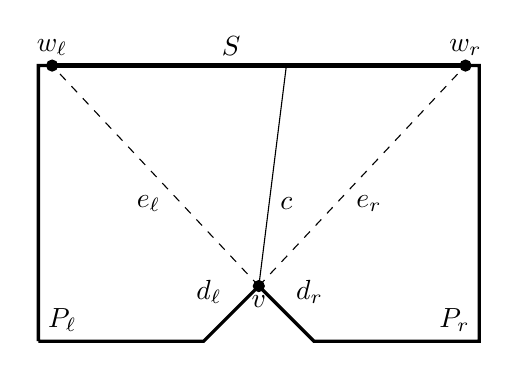
\begin{tikzpicture}[scale=0.7]
		\coordinate (x_0) at (0.25,5);
		\coordinate (x_1) at (7.75,5);

		\draw [very thick] (0,0)--(3,0)--(4,1)--(5,0)--(8,0)--(8,5)--(0,5)--(0,0);
		\draw [dashed] (4,1)--(x_0);
		\draw [dashed] (4,1)--(x_1);
		\draw [ultra thick] (x_0)--(x_1);
		\draw (4,1)--(4.5,5);

		\draw [fill] (4,1) circle [radius=0.1] node [below] {$v$};
		\draw [fill] (x_0) circle [radius=0.1] node [above] {$w_{\ell}$};
		\draw [fill] (x_1) circle [radius=0.1] node [above] {$w_r$};
		
		\node [above right] at (0,0) {$P_{\ell}$};
		\node [above left] at (8,0) {$P_r$};
		\node [above] at (3.5,5) {$S$};
		\node at (2,2.5) {$e_{\ell}$};
		\node at (6,2.5) {$e_r$};
		\node at (4.5,2.5) {$c$};
		\node [above left] at (3.5,0.5) {$d_{\ell}$};
		\node [above right] at (4.5,0.5) {$d_r$};

	\end{tikzpicture}
	\caption{Decomposing cut originating at a reflex vertex.}
	\label{fig:cut}
\end{figure}


\section{Traveling Salesman Problem Preliminaries}
\label{section:GTSP}

A graph $G$ is defined by a pair of sets $G=(V,E)$, where $V$ is a set of vertices in the graph and $E$ is a set of edges between the vectices. An edge connecting vertices $u$ and $v$ exists in the graph if there is a pair $\{u,v\}$ in $E$. A graph is complete if there exist a pair $\{u,v\}$ for every $u,v\in V, u\neq v$. An example of a complete graph is shown in Figure~\ref{fig:complete_graph}.
\begin{figure}
	\centering
	\subfile{img/chapter_3/graph}
	\caption{An example of a complete graph $G$.}
	\label{fig:complete_graph}
\end{figure}

\begin{definition}[Weighted Graph]
	A graph $G$ is weighted if for every edge $e_i\in E$, there exists a value $w_i>0$.
\end{definition}
\begin{definition}[Subgraph]
	A subgraph $\mathcal{G}=(V_S,E_S)$ of a graph $G=(V,E)$ is a graph where $V_S\subseteq V$ and $E_S\subseteq E$. The subgraph is a spanning subgraph when $V_G=V$.
\end{definition}
\begin{definition}[Cycle]
	A cycle $C$ in graph $G$ is a sequence of vertices $v_1,v_2,\ldots,v_k$, such that there is no repeating vertices in the sequence and no repeating edges. The last edge of a cycle is an edge between $v_1$ and $v_k$. 
\end{definition}
\begin{definition}[Tour]
	A cycle on a spanning subgraph is called a tour.
\end{definition}

\begin{problem}[TSP]
Given a complete weighted graph $G=(V,E,w)$, compute a tour $T$ of $G$ such that the sum of edge weights is minimized. An example of a TSP tour is shown in Figure~\ref{fig:tsp_tour}.
\end{problem}

\begin{figure}
	\centering
	\subfile{img/chapter_3/tsp_tour}
	\caption{An example of a TSP tour on a complete graph $G$.}
	\label{fig:tsp_tour}
\end{figure}

\begin{figure}
	\centering
	\subfile{img/chapter_3/gtsp_tour}
	\caption{An example of a GTSP tour on a complete graph $G$.}
	\label{fig:gtsp_tour}
\end{figure}

Another important problem is called the Generalized Traveling Salesman Problem (GTSP). It is defined over a complete graph and a vertex partition. A vertex partition is a set of disjoint subsets of $V$, $\{V_1,V_2,
\ldots,V_m\}$.
\begin{problem}[GTSP]
Given a complete graph $G=(V,E,w)$ and a vertex partition $\{V_1,V_2,\ldots,V_m\}$, compute a tour of $G$ that includes exactly one vertex from each subset $V_i$ and the sum of edge weights is minimized. An example of a GTSP tour is shown in Figure~\ref{fig:gtsp_tour}.
\end{problem}

A TSP problem is known to be NP-hard. A GTSP problem can be solved as a reduction to a TSP problem~\cite{noon1993efficient}. However, there are numerous approximate and suboptimal solutions available. One of them is a solver called GLKH, which utilizes a Lin-Kernighan TSP heuristic~\cite{helsgaun2009general}. In this thesis, we utilize the GLKH solver for solving GTSP problems.

%\section{Contours Introduction}
%\label{section:background_contours}

%In this section, the concept of contours is introduced and some of the related material in medial axis and straight skeletons is reviewed.

%Blum~\cite{blum1967transformation} in 1967 have proposed a notion of medial axis as a shape description. The motivation behind this was generation of ways to represent a shape. The medial axis is defined as follows.
%\begin{definition}
%Suppose a simple polygon $G$ is given then the medial axis $M(G)$ is a set of points $\{q\}$ in the interior of $G$ such that there are at least two points on the object's boundary that are equidistant from $\{q\}$ and are closest to $\{q\}$.
%\end{definition}
%There is an associated radius function that maps every points on $M(G)$ to a radius. This radius specifies the distance of each points on the axis to the boundary. This allows for reconstruction of the original shape by looking at the union of circles centered at each point of $M(G)$ with the corresponding radius. Lee~\cite{lee1982medial} have proposed a $\mathbb{O}(b\log n)$ algorithm for computing medial axis where $n$ is the number of edges.

%Related to medial axis is the concept of straight skeletons introduced by Aichholzer~\cite{aichholzer1996novel}. Because of its structure, it can be misconstrued to be equivalent to medial axis. However, even though, for convex polygons they are identical, the difference arise at the reflex vertices of a polygon. The straight skeleton are defined in terms of a shrinking process where all points on the boundary of a polygon are moving inwards with the same speed. In the process there are two events that can happen. The first event is the edge event. This is where an edge is reduced to zero length in the process of shrinking resulting in its two adjacent edges be adjacent to each other instead. The second event is a split event where the polygon is split into two. Reflex vertices result in this type of event. 
%During the shrinking process, a set of nested polygons is generated. These are of particular interest with respect to this work.

%The straight skeleton is defined as the union of the pieces of angular bisectors traced out by polygon vectices as they are shrinked.
\end{document}